The code for the instructions below is in GitHub repository:
\begin{itemize}
    \item \textit{models$\setminus$random\textunderscore cut\textunderscore forest$\setminus$rcf\textunderscore bmw\textunderscore train\textunderscore deploy.ipynb} - the notebook contains a set of scripts to train and deploy the RCF model
    \item \textit{models$\setminus$random\textunderscore cut\textunderscore forest$\setminus$rcf \textunderscore test\textunderscore endpoint\textunderscore model.ipynb} - the notebook contains a set of scripts to test the deployed model
\end{itemize}
Amazon Sagemaker RCF is an algorithm designed to detect anomalous data points within a dataset. 
This section describes a creation and a deployment of a SageMaker RCF model. 
The data consists of a number of requests (VPC Flowlogs from BMW) aggregated into one minute buckets. To train the model, we used the data over the course of one week that represents a normal pattern. Then, we fed the whole data into the trained model for testing.\\To start with, it is necessary to specify the locations where we will store our training data and trained model artifacts. In particular, we need the following data:
\begin{itemize}
    \item bucket - An S3 bucket accessible by an account.
    \item prefix - The location in the bucket where a notebook's input and output data will be stored. (The default value is sufficient.)
\end{itemize}
\begin{figure}[h]
    \centering
    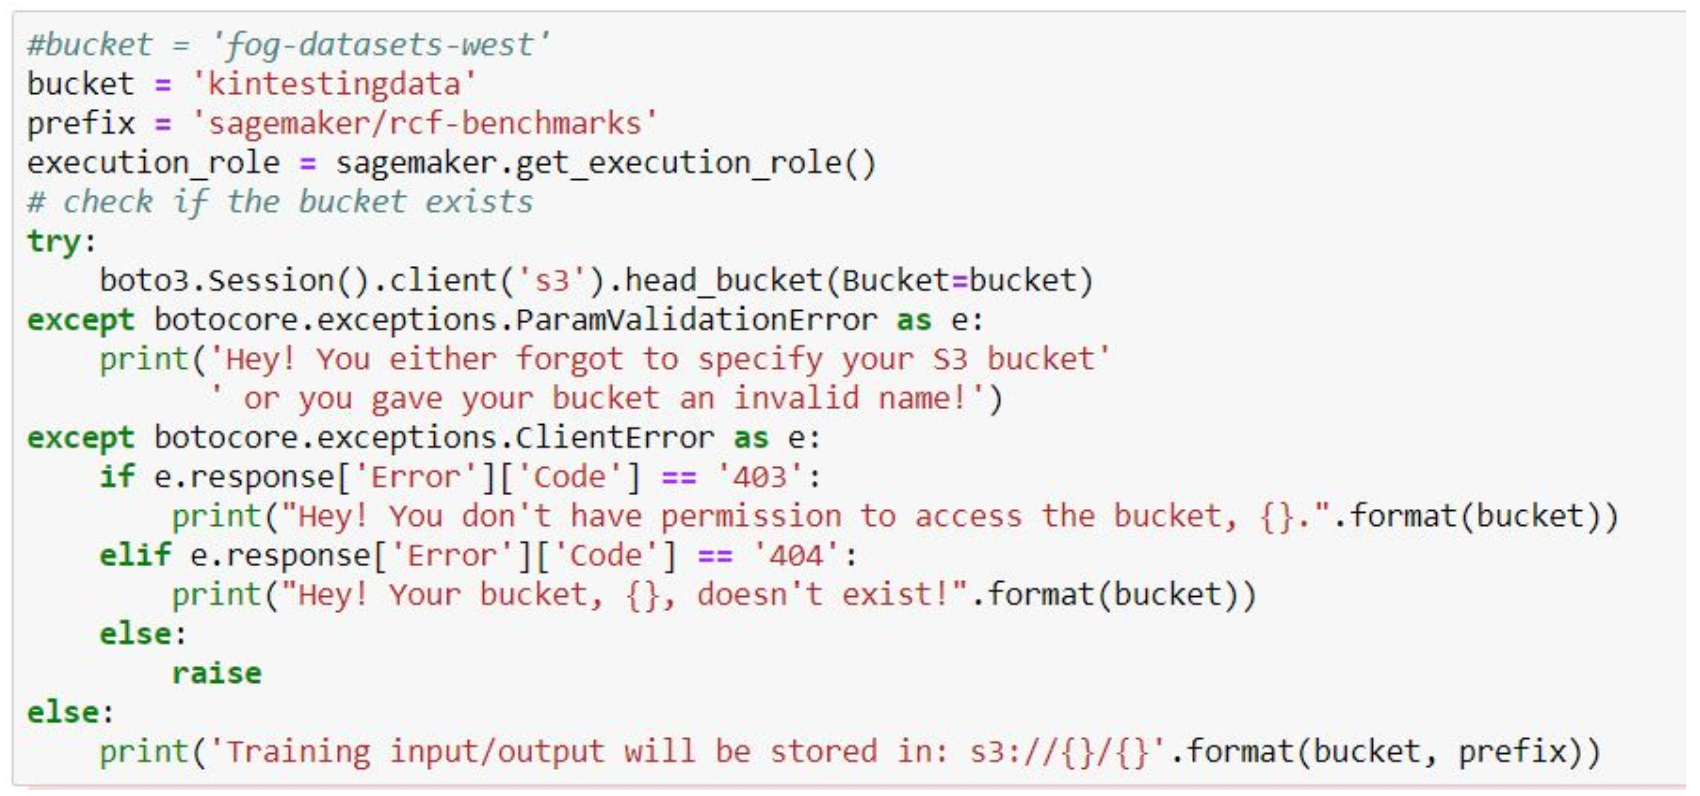
\includegraphics[width=1\textwidth]{images/rcf-data-location.png}
    \caption{Specifications for data location}
    \label{fig:rcf_data_location}
\end{figure}
Next, we configure a SageMaker training job to train the Random Cut Forest (RCF) algorithm on one minute data.

\textbf{Hyperparameters}\\
Particular to a SageMaker RCF training job are the following hyperparameters:
\begin{itemize}
    \item \textit{num\textunderscore samples\textunderscore per\textunderscore tree} - the number of randomly sampled data points sent to each tree. As a general rule, 1/\textit{num\textunderscore samples\textunderscore per\textunderscore tree} should approximate the estimated ratio of anomalies to normal points in the dataset.
    \item \textit{num\textunderscore trees} - the number of trees to create in the forest. Each tree learns a separate model from different samples of data. The full forest model uses the mean predicted anomaly score from each constituent tree.
    \item \textit{feature\textunderscore dim} - the dimension of each data point.
\end{itemize}
Along with these RCF model hyperparameters, we provide additional parameters defining things like the EC2 instance type on which training will run, the S3 bucket containing the data, and the AWS access role. Note that,
\begin{itemize}
    \item Recommended instance type: ml.m4, ml.c4, or ml.c5
    \item Current limitation: The RCF algorithm does not take advantage of GPU hardware.\footnote{ https://docs.aws.amazon.com/sagemaker/latest/dg/randomcutforest.html}\\
\end{itemize}
\begin{figure}[h]
    \centering
    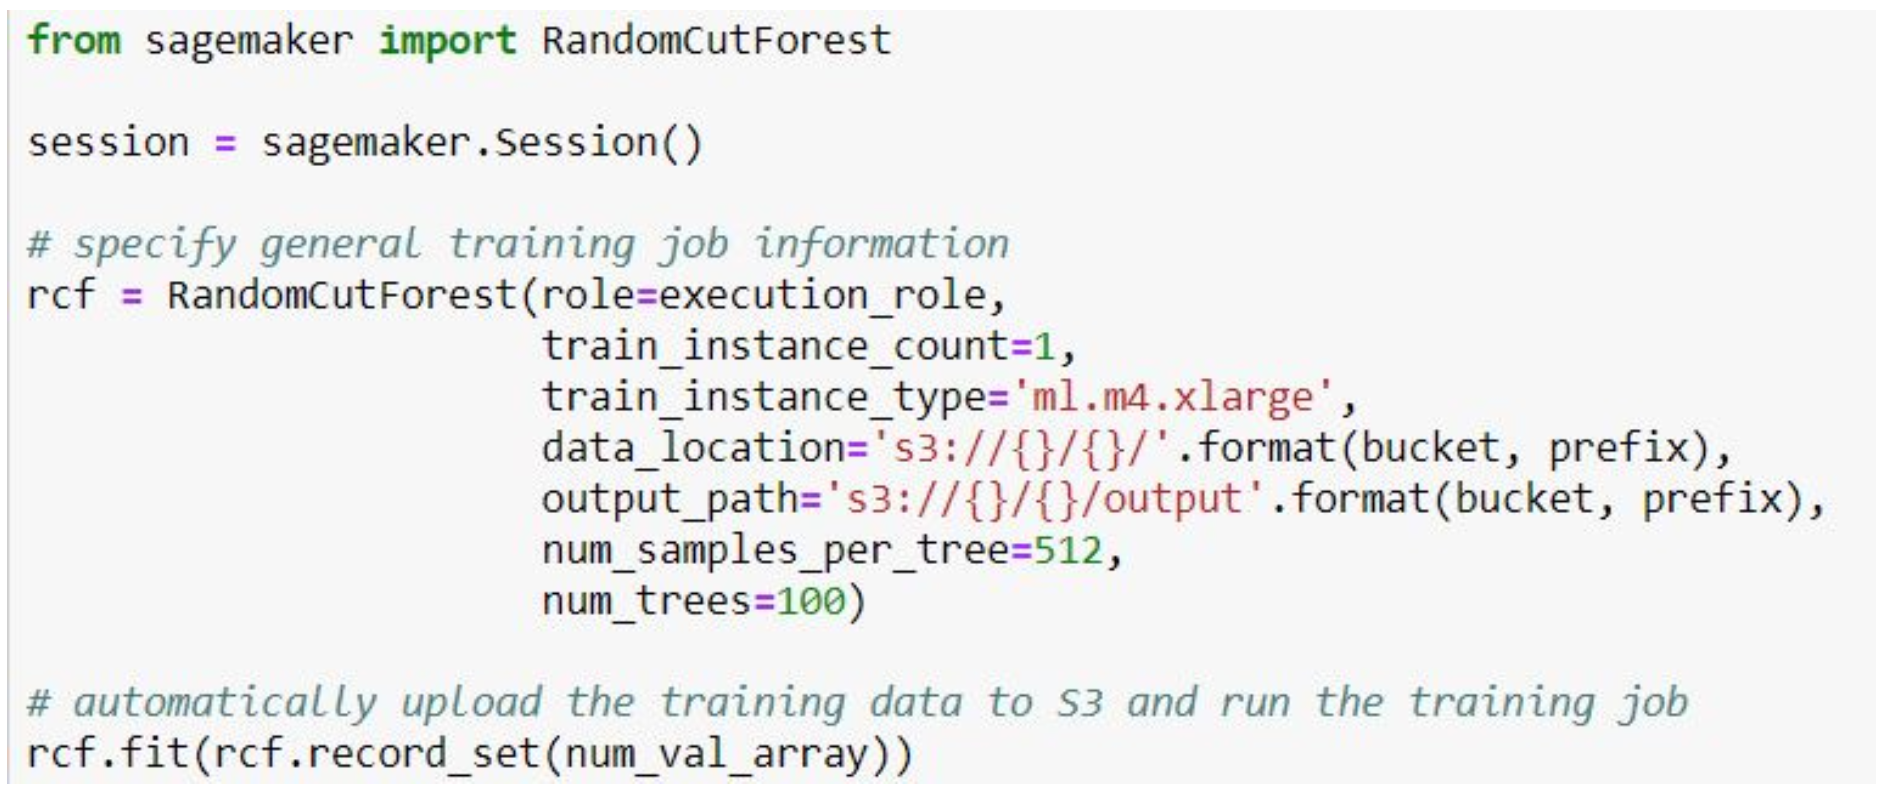
\includegraphics[width=1\textwidth]{images/rcf-model-training.png}
    \caption{RCF Model training}
    \label{fig:rcf_model_training}
\end{figure}
We used SageMaker Python SDK deploy() function from the job to create an inference endpoint. The function has two input parameters:  the instance type and an initial number of instances. 

There are two ways to invoke the trained model:
\begin{itemize}
    \item Right after training in the same notebook, calling a job’s \textit{predict(Test\textunderscore data)} function
    \item From elsewhere(e.g., inside a lambda function), using a function \textit{runtime.invoke\textunderscore endpoint\\(EndpointName, ContentType, Body)}
\end{itemize}
The model outputs an anomaly score for each input data point. It is suggested in a RCF documentation, to compute a value of the anomaly threshold as 3 standard deviations from the mean score. Any value that is beyond the threshold is considered as an anomaly. 
The way to compute the threshold value is subject to change. Depending on business requirements, one can calculate it either once for the whole period of data, or for shorter periods of time, e.g., recompute threshold every day.\\We decided to experiment and calculate the threshold per each day and these results are available below.
The first following plot represents the data, the second one demonstrates testing results. The red plot depicts threshold values that we compute for each day. As we can see, not only high local peaks are detected as anomalies, but also local downfalls and congestions on bottoms are anomaly candidates. 
\begin{figure}[h]
    \centering
    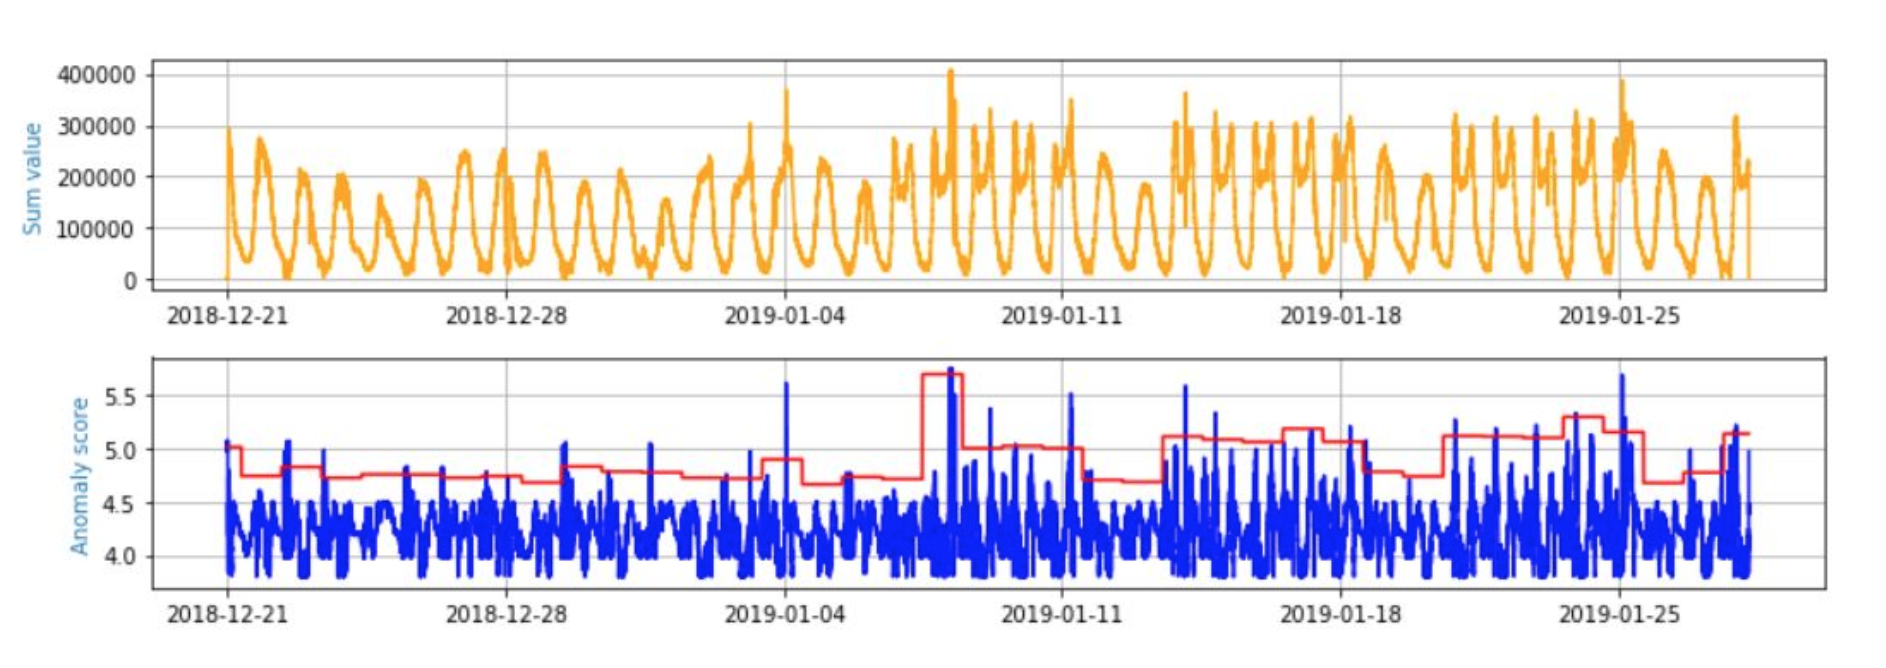
\includegraphics[width=1\textwidth]{images/rcf-results.png}
    \caption{Plotted data, anomaly scores, and anomaly threshold values}
    \label{fig:rcf_results}
\end{figure}
\FloatBarrier


